\begin{tikzpicture}
\node[inner sep=0pt] (obrazek) at (0,0)
    {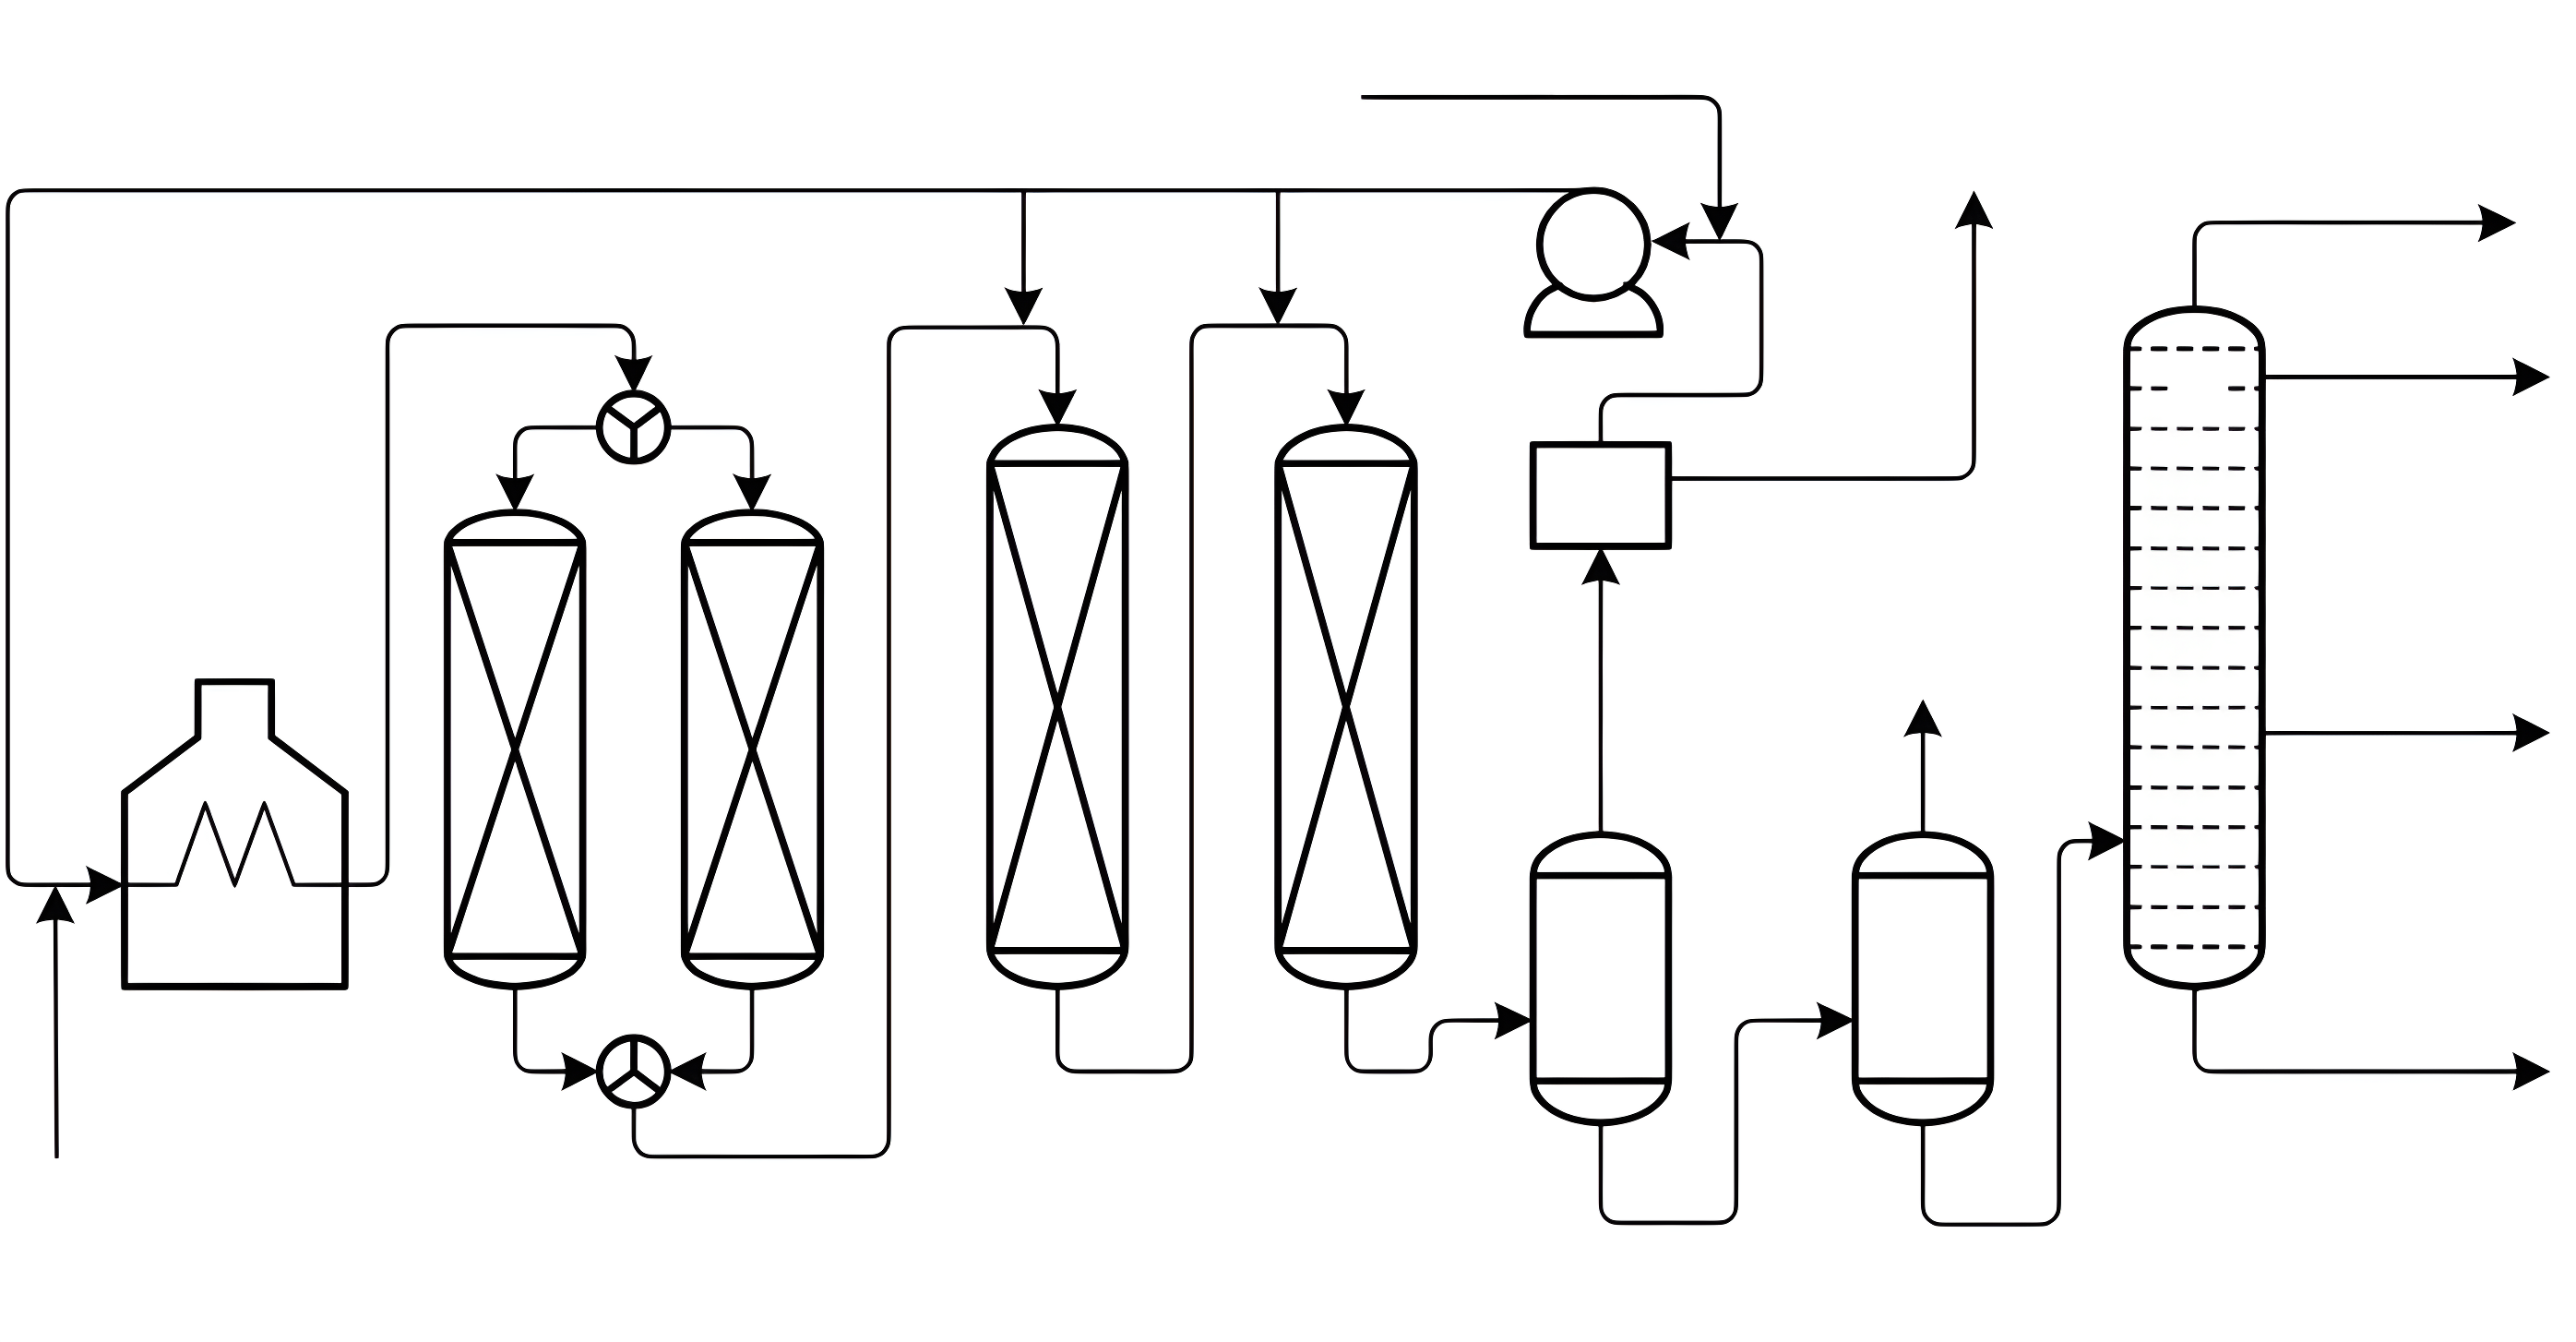
\includegraphics[width=0.8\textwidth]{figures/hydrokrak_Pschema.png}};
\node[font=\small\bfseries] at (-4.57,-1.15) {1};
\node[font=\small\bfseries] at (-3.37,0.317) {2};
\node[font=\small\bfseries] at (-2.3,0.32) {2'};
\node[font=\small\bfseries] at (-1,0.646) {3};
\node[font=\small\bfseries] at (0.25,0.65) {3};
\node[font=\small\bfseries] at (1.35,-1.15) {4};
\node[font=\small\bfseries] at (2.765,-1.15) {5};
\node[font=\small\bfseries] at (3.95,1.22) {6};
\node[font=\small\bfseries] at (1.35,0.77) {7};
\node[font=\small\bfseries] at (1.32,1.85) {8};

\node[font=\scriptsize] at (-2.9,2.3) {\ce{H2}}; % mezi 2 a 2'

\node[font=\small] at (-4.55,-1.97) {surovina};
\node[font=\small] at (-0.6,2.5) {čerstvý \ce{H2}};
\node[font=\small,align=center] at (1.9,-0.3) {recykl\\\ce{H2}};
\node[font=\small] at (2.9,0.15) {plyny};
\node[font=\small,align=center] at (2.9,2.5) {kyselé\\plyny};

\node[font=\small] at (4.8,2.2) {plyny};
\node[font=\small] at (4.8,1.55) {benzin};
\node[font=\small,align=left] at (4.95,0.2) {plynový\\olej};
\node[font=\small,align=left] at (4.65,-2.3) {nízkosirný\\těžký olej};

\end{tikzpicture}